\documentclass[11pt, oneside]{article}   	% use "amsart" instead of "article" for AMSLaTeX format
\usepackage{geometry}                		% See geometry.pdf to learn the layout options. There are lots.
\geometry{letterpaper}                   		% ... or a4paper or a5paper or ... 
%\geometry{landscape}                		% Activate for rotated page geometry
%\usepackage[parfill]{parskip}    		% Activate to begin paragraphs with an empty line rather than an indent
\usepackage{graphicx}				% Use pdf, png, jpg, or eps§ with pdflatex; use eps in DVI mode
								% TeX will automatically convert eps --> pdf in pdflatex		
\usepackage{amssymb}

%SetFonts

%SetFonts
\setlength{\parindent}{0pt}

\title{Summary of a simple deep learning model for stock price prediction using TensorFlow by Sebastian Heinz}
\author{Jody Shu}
%\date{}							% Activate to display a given date or no date

\begin{document}
\begin{Large}
\maketitle
%\section{}
%\subsection{}

This article introduces a high level approach to predict stock price using TensorFlow package in Python.  The author has a link to his dataset, but unfortunately, the link is no longer available, but since the purpose of this summary is to understand this paper and how he coded the Python, I will ignore it and use my own data in the future for application.

The dataset is also spiltted into training and test data set which 80$\% \ being\ training \ and \ 20\%$ for test data.\\As similar to other papers I summaried for homework 6, the author uses MinMaxScaler package to scale the training set and test set separately. Moreover, there are four hidden layers, and started out with 1024 neurons and half the size in the subsequent layer until the 4th layer which is 128 neurons.  Basically that is each two input data produces one output, and use that output as input for the subsequent layer.  And then the author continues to talk about the setup of the bias and weight.  For example, the second dimension (argument) of the previous layer is the first dimension of the current layer for weight matrices.  In addition, the biases argument is the second argument of the current layer's weight matrix.\\

Next, the author discusses about the hidden layer activation functions.  There are many activation functions, and in this tutorial, the rectified linear unit (ReLU) is used in the example.  The network architecture is a feedforward network.  Further more, the author used mean squared error function between the true and prediction as the cost function and to minimize the cost function, the Adaptive Moment Estimation (Adam) optimizer is used.  
The whole procedure starts training the data by batches feed through the network until it reaches the output layer, and TensorFlow compares the output against the true, and then optimized and updates the weights and biases accordingly, and the procedure continues until all batches have been presented to the network which is called an epoch.  The algorithm stops when the maximum number of epochs is reached.  Once training set is done, the model can be evaluated by the test set.  The result for the final test MSE is 0.00078 which is very low and the mean absolute percentage error of the forecast is 5.31$\%$ which is pretty good.









%be an introduction on how to use neural networks to predict the stock market, in particular the price of a stock (or index).  \\
%
%The author follows the step from data acquisition, data preprocessing (split up into train and test set, and each window size has sample size 10).  After that, the author use multiplayer perceptron (MLP) and the Long Short Term Model (LSTM).  The different between MLP and LSTM is that MLP has no ability to analyze the relationship between batch of data and LSTM has the ability to store certain information about the data for later use.  LSTM is a special kind of Recurrent Neural Networks (RNNs).  In a general RNNs, there is a problem which is that it suffers from the vanishing gradient problem because as the layers increase, the gradient decrease.  However, this problem is solved by using LSTMs.
%
%The author implement the LSTMs/MLP by using keras Python package which adding layers to the network instead of defining the entire network at once.  The author normalizes the data by divide it by 200, so the weights in the neural network do not grow too large.  The Adam optimizer is chosen because it takes advantages of Root Mean Square Propagation and Adaptive Gradient Algorithm.  After that, the author feed the training data into the model, and use test data to evaluate how well the model perform after it is trained.  Once the author evaluate the test data, he used a new set of data and run the algorithm and 'backtesting the Model', and the prediction stock price is pretty good as you can see the graph below.  
%
%\begin{figure}[h] %  figure placement: here, top, bottom, or page
%   \centering
%   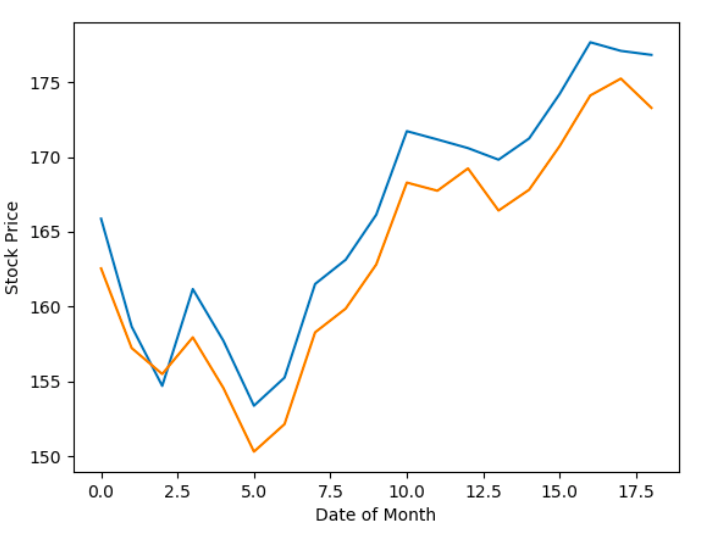
\includegraphics[width=6in]{prediction_plot} 
%\end{figure}


\end{Large}
\end{document}


